\chapter{生物信息学与中医药的交叉融合 \\ ——中医药定量研究的数据科学和统计学方法}

\begin{center}
  作者:洪宇睿
\end{center}

\section*{摘要}
\begin{center}
  
  本调研报告聚焦于生物信息学与中医药交叉融合的研究领域,特别是中药化合物组分的初步数据收集与调研。在当前中医药研究中,化合物的定量数据不够完善,限制了药材鉴别和基于机器学习的处方优化的进展。本研究基于不同文献中的中药化合物数据,探讨了这些数据共同涉及的化合物,以评估基于现有文献的定量研究的可行性。通过对公开文献中的化合物定量数据进行初步收集与分析,本研究揭示了现有研究对化合物定量信息的收集和呈现方式不利于开展数据增强的现状,强调了进一步完善中药化合物定量数据的重要性,提供了利用现有数据进行对比分析的初步思路,为中医药定量研究提供了新的视角和方法。

\end{center}
\textbf{关键词:生物信息学;中医药;化合物定量;数据科学}

\section{研究背景}

中医作为一种历史悠久的医学体系,在现代医学领域逐渐受到重视。然而,中医药的研究与发展面临着一些固有的挑战。本研究背景部分将围绕中药材的化合物组分定量研究,探讨现有研究的局限性、挑战以及可能的解决途径。

中药的定量研究包括临床药代动力学、药材成分配比的质量检测、处方优化等多个方面。尽管这些研究为中医药的现代化发展提供了支持,但是对于药材与其效用之间准确的映射关系,尤其是基于古籍和临床实践的处方中药物作用的定量研究,仍然相对缺乏。这种研究的不足虽然有中医药的理论体系独特,涉及的药用成分极为复杂的客观原因,但也限制了中医药的研究验证,导致其长于“守正”而短于“创新”。\cite{Chen_Bi_Xie_Zhang_Shi_Guo_Yin_Zhang_Xin_Song_2021}

对于中药的化合物组分的定量研究,尤其是对于重要化合物的定量研究,目前仍然存在很多问题,如数据不完善、不可用、不可靠;现有关键组分的定量研究过程,往往依赖大量的临床记录首先确定关键药材,然后通过化学方法分离进行验证,这种方法在现有的临床数据支持下往往只能发现成分效果极其明显的单一药材,而对于往往由多种药材组成的复方,这种方法往往无法发现其中共同作用的关键组分。这些问题导致了中医药的定量研究的发展受到了很大的限制。\cite{Chu_Sun_Huang_Peng_Zhou_Zhang_2020}

进行大规模实验以定量刻画中药材化合物含量是解决上述问题的途径之一,但这种方法需要大量的资源和成本投入,使得研究实施变得复杂。为了解决高质量数据缺乏的问题,从公开文献中收集中医药信息成为一种可行的方法,这也是本调研的主要内容。在这个过程中,我们面临的主要挑战包括文献质量不一、数据组织形式不统一、化合物涉及范围有限、以及数据缺失问题。这些问题需要通过细致的数据清洗和增强来解决。

中药材的化合物组分受到生长环境、采收时间、加工方法等因素的影响,即使是同一品种的药材,其化合物含量也存在显著差异。这不仅是建立中药材化合物组分定量数据库的挑战,也是一个研究机遇。我们可以利用这种差异作为研究的突破点,将不同生长环境的中药材之间的含量差别作为同一物种的组内差别,从而更好地确定不同药材的组间差别,搜索药材的关键特征。

\section{研究方法}

\subsection{数据收集}

我们预期的完整结果是得到包括600余种中药材的化合物组分定量数据库,每组尽可能多地包含化合物的定量信息,包括尽可能广的化合物种类、不同文献对同一化合物组分的定量结果,以及同一篇文献对同一药材同一化合物所作的重复。其中,组内重复的主要形式有文献原始数据对同一植物物种的指定药用部位的重复、包含标准差的化合物均值,以及可视为不同批次的,同属异种或者同属同种不同亚种的药材的重复。在数据收集阶段,这些往往是我们能从文献中直接得到的结果。

具体的数据收集任务可以分为如下几个步骤:

\begin{itemize}
  \item 使用药材名或专有拉丁名称,或者植物学名,在文献数据库中搜索相关文献,并根据文章语义在文献中定位化合物定量数据。在此步骤中,可以依据目标数据集质量和规模的平衡,筛选特定期刊、影响因子等的文献。
  \item 根据具体的数据呈现形式进行数据处理。具体而言,一部分论文的补充材料中直接含有xlsx或者csv格式的原始数据;在线论文中的HTML数据表格可通过Table Converter Online等转换工具得到表格文件;对于只有PDF格式的文献,可以借助Mathpix Snipping Tool等OCR工具进行转换。
  \item 对于原始数据进行数据清洗。主要需要将数据中的单位统一,对含有标准差的均值记录标准差、样本容量以便后续重建分布,以及将原始宽数据转化为长数据,以便后续分析。
\end{itemize}

例如,对以下的数据表格:

\begin{figure}[H]
  \centering
  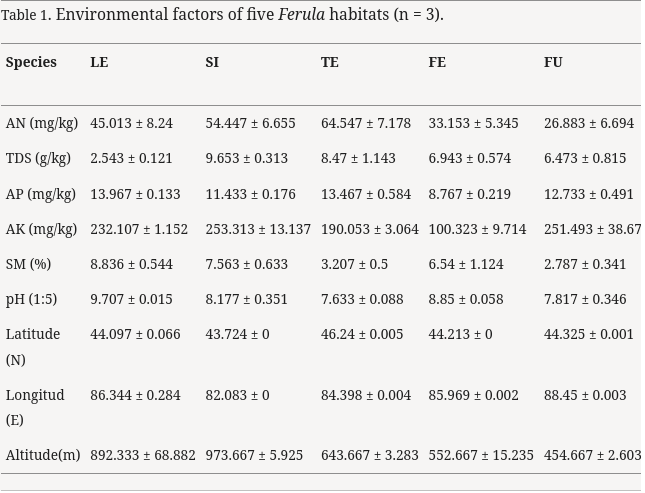
\includegraphics[width=0.8\textwidth]{figures/fig1.png}
  \caption{原始数据表格\cite{Jiang_Lan_Peng_Wang_Zhuang_2023}}
  \label{fig:fig1}
  常见的原始数据表格类型,其中除了含量信息(AN, TDS, AP, AK, SM),还包括一些对数据收集而言多余的列;组织形式为长数据,即不同种(LE, SI, TE, FE, FU)作为不同的数据列,需要转化成行长数据,即设置一个“学名”列,将不同种的数据均作为同一个表格中的记录,以“学名”列来标记所属。
\end{figure}

假设以$\mathrm{mg/kg}$作为统一的单位,经过Table Converter Online转换后及一些手动调整后,初步得到:

\begin{table}[H]
  \centering
  \begin{tabular}{|l|l|l|l|l|l|}
  \hline
      Species & LE & SI & TE & FE & FU \\ \hline
      AN & 45.013±8.24 & 54.447±6.655 & 64.547±7.178 & 33.153±5.345 & 26.883±6.694 \\ \hline
      TDS & 2543±121 & 9653±313 & 8470±1143 & 6943±574 & 6473±815 \\ \hline
      AP & 13.967±0.133 & 11.433±0.176 & 13.467±0.584 & 8.767±0.219 & 12.733±0.491 \\ \hline
      AK & 232.107±1.152 & 253.313±13.137 & 190.053±3.064 & 100.323±9.714 & 251.493±38.673 \\ \hline
  \end{tabular}
\end{table}

使用如下的R代码将其转化为长数据,并将标准差信息从均值中分离出来,添加上样本容量信息:

\lstset{basicstyle=\ttfamily, keywordstyle=\color[RGB]{40,40,255}, breaklines}

\begin{lstlisting}[language=R]
library(tidyverse)

# Read data
df <- read.csv("input.csv", header = TRUE, stringsAsFactors = FALSE)

# Convert wide data to long format, order by batch
df_long <- df %>%
  pivot_longer(
    cols = -Species, 
    names_to = "species", 
    values_to = "value"
  ) %>%
  mutate(
    batch = match(species, names(df)[-1]),
    compound = Species
  ) %>%
  select(batch, species, compound, value) %>%
  arrange(batch)

# Function to split mixed data into mean and std
split_data <- function(x) {
  parts <- strsplit(x, "±", fixed = TRUE)[[1]]
  mean <- as.numeric(trimws(parts[1]))
  std <- as.numeric(trimws(parts[2]))
  return(c(mean, std))
}

# Apply the function and create new columns
df_long <- df_long %>%
  mutate(
    mean = sapply(value, function(x) split_data(x)[1]),
    std = sapply(value, function(x) split_data(x)[2]),
    size = 3
  ) %>%
  select(-value)

# Output the result
write.csv(df_long, "output.csv", row.names = FALSE)
\end{lstlisting}

可以得到如下的长数据结果,这样就可以与其他文献中有关这一种中药的数据进行合并;收集到足够批次后,可以在数据中额外添加一个此药材的标签,再与其他药材的数据合并。这样就得到了格式严谨,既便于研究者阅读维护又便于计算机读取操作的化合物含量信息:

\begin{table}[H]
  \centering
  \begin{tabular}{|l|l|l|l|l|l|}
  \hline
      "batch" & "species" & "compound" & "mean" & "std" & "size" \\ \hline
      1 & "LE" & "AN" & 45.013 & 8.24 & 3 \\ \hline
      1 & "LE" & "TDS" & 2543 & 121 & 3 \\ \hline
      1 & "LE" & "AP" & 13.967 & 0.133 & 3 \\ \hline
      1 & "LE" & "AK" & 232.107 & 1.152 & 3 \\ \hline
      2 & "SI" & "AN" & 54.447 & 6.655 & 3 \\ \hline
      2 & "SI" & "TDS" & 9653 & 313 & 3 \\ \hline
      2 & "SI" & "AP" & 11.433 & 0.176 & 3 \\ \hline
      2 & "SI" & "AK" & 253.313 & 13.137 & 3 \\ \hline
      3 & "TE" & "AN" & 64.547 & 7.178 & 3 \\ \hline
      3 & "TE" & "TDS" & 8470 & 1143 & 3 \\ \hline
      3 & "TE" & "AP" & 13.467 & 0.584 & 3 \\ \hline
      3 & "TE" & "AK" & 190.053 & 3.064 & 3 \\ \hline
      4 & "FE" & "AN" & 33.153 & 5.345 & 3 \\ \hline
      4 & "FE" & "TDS" & 6943 & 574 & 3 \\ \hline
      4 & "FE" & "AP" & 8.767 & 0.219 & 3 \\ \hline
      4 & "FE" & "AK" & 100.323 & 9.714 & 3 \\ \hline
      5 & "FU" & "AN" & 26.883 & 6.694 & 3 \\ \hline
      5 & "FU" & "TDS" & 6473 & 815 & 3 \\ \hline
      5 & "FU" & "AP" & 12.733 & 0.491 & 3 \\ \hline
      5 & "FU" & "AK" & 251.493 & 38.673 & 3 \\ \hline
  \end{tabular}
\end{table}

\subsection{基于共有化合物的药材比对分析能力预测}

在这里,我们收集了刺五加等10种中药材的化合物含量信息(出于课题组的保密要求,具体表格未在这里给出),运用如下的代码检查了这些药材之间共有化合物的情况:

\begin{lstlisting}
suppressMessages(library(dplyr))
library(readxl)
options(tibble.print_max = Inf)
df <- read_excel('input.xlsx')

find_common_compounds_first_occurrence <- function(df) {
  # Add a column with row number to keep track of the original order
  df <- df %>% mutate(Row_Order = row_number())
  
  # Group by 'Compound' and 'Article_DOI', then summarize the first occurrence
  compound_first_occurrence <- df %>%
    group_by(Compound, Article_DOI, Latin_Name) %>%
    summarise(First_Occurrence = first(Row_Order)) %>%
    ungroup() # Ungroup to allow for the next operations
  
  # Count the number of unique DOIs for each compound
  compound_counts <- compound_first_occurrence %>%
    group_by(Compound) %>%
    summarise(Count = n_distinct(Article_DOI)) %>%
    filter(Count > 1) %>%
    select(Compound) # Select the compounds that appear in more than one paper
  
  # Join with the first occurrences
  common_compounds_first_occurrence <- compound_first_occurrence %>%
    inner_join(compound_counts, by = "Compound")
  
  return(common_compounds_first_occurrence)
}

common_compounds_first_occurrence <- find_common_compounds_first_occurrence(df)
print(common_compounds_first_occurrence)  
\end{lstlisting}


根据输出结果,共发现6种存在于两种药材中的具体化合物。假设任意两种药材之前出现相同化合物的种类期望是$\mathrm{E}$,则在数据集规模为$\mathrm{N}$时,新增的共享化合物配对数的期望可以用$\mathrm{NE}$来表示,这样,我们就可以求和得到规模$\mathrm{N}$的数据集所含的共享化合物配对数期望与为$\frac{N(N-1)}{2}E$,即与数据集规模的平成正比;平均每中药材与其他药材共享化合物的配对数期望为$(N-1)E$,即会线性增长,代入我们前10组数据得到的实际配对数,可以估计当数据集的规模为600时,每个化合物的平均配对数将达到80左右,药材的化合物组成将具有较高的交叉性。这种高度的交叉性为使用机器学习方法探究中药材的特征化合物提供了理论基础。通过统计不同药物之间出现相同化合物的组数,我们可以跨药材验证特定化合物是否可以作为区分两种或多种药材的关键指标。这种方法有助于深入理解中药材的化学特性和药效关系。

\subsection{基于方差分析的化合物特征性判断}

在得到数据集后,我们可以具体考察每一对含有公共化合物的药材,应用方差分析(ANOVA)来检验两组数据是否存在统计学上的显著差异,以判断这种公共化合物的含量是否可以成为区分这两种中药材的可靠特征。例如,在对岩白菜(BERGENIAE RHIZOMA)和枇杷叶(ERIOBOTRYAE FOLIUM)这两种中药中儿茶素(Catechin)含量的研究中,我们发现岩白菜的5个样本含量分别为2.4000\%,1.1300\%,2.0000\%,3.3100\%,2.8600\%\cite{Pandey_Kumar_Meena_Srivastava_Mishra_Tiwari_Pal_Nair_Upreti_Rana_2017},而枇杷叶的2个样本含量为1.2040\%和0.7344\%\cite{Chen_Zhang_Chen_2008},我们便可以检验儿茶素的含量是否可以区分这两种中药材。

应用现有成熟统计工具,的我们将使用单因素方差分析(One-Way ANOVA),它是一种统计技术,用于比较两个或多个样本均值是否存在显著差异,而不必进行多个两样本t检验。在单因素ANOVA中,我们假设所有组的总体均值相等,这是零假设(H0)。替代假设(H1)则是至少有一个组的均值与其他组不同。ANOVA通过比较组内方差(样本内部的变异)与组间方差(不同样本均值之间的变异)来决定是否拒绝零假设。

对于上面这个具体例子,我们运行以下的代码:

\begin{lstlisting}
bergeniae <- c(2.4000, 1.1300, 2.0000, 3.3100, 2.8600)
eriobotryae <- c(1.2040, 0.7344)
catechin_content <- c(bergeniae, eriobotryae)
herb_type <- factor(rep(c("Bergeniae", "Eriobotryae"),
                    times = c(length(bergeniae), length(eriobotryae))))
catechin_anova <- aov(catechin_content ~ herb_type)
summary(catechin_anova)

Df Sum Sq Mean Sq F value Pr(>F)  
herb_type    1  2.684   2.684   4.621 0.0843 .
Residuals    5  2.905   0.581                 
---
Signif. codes:  0 ‘***’ 0.001 ‘**’ 0.01 ‘*’ 0.05 ‘.’ 0.1 ‘ ’ 1
\end{lstlisting}

P值大于0.05但小于0.1,这意味着我们没有足够的证据在95\%的置信度下拒绝原假设。然而,这个P值落在了0.05到0.1之间,这在统计学上是一个边缘值,可以认为是有趋势性的证据表明两种药材中儿茶素含量存在差异,但这个证据不够强以确立显著性。在一些情况下,研究者可能会考虑接受更高的错误率(例如10\%),此时,我们可以说有显著性的趋势表明儿茶素含量可以作为区分这两种药材的特征。因此,我们要进行更多这样的方差分析来决定是否对数据集应用这样的策略,或者依然采用保守的0.05的P值门槛,认为根据ANOVA的结果,我们不能坚定地说儿茶素含量是区分岩白菜和枇杷叶的可靠特征。

目前的ANOVA是直接基于原始数值进行的,没有考虑样本量和标准差。如果我们有每个样本的标准差和样本量信息,我们可以采取以下额外的步骤来增强我们的分析:

\begin{itemize}
\item   \textbf{加权ANOVA}:当组间样本量差异较大时,使用加权均方和加权F值可以更准确地反映组间的差异。
\item   \textbf{元分析方法}:如果每个样本的标准差已知,可以应用元分析方法来综合考虑不同研究的结果,这在跨研究进行综合分析时尤其有用。
\item   \textbf{方差稳定性分析}:考虑到方差的稳定性是进行ANOVA的前提条件,如果每个样本的标准差已知,可以先进行方差齐性检验,如Levene's test或Bartlett's test。
\item   \textbf{数据分布重建}:通过均值和方差重建每个样本的数据分布(如假设数据服从正态分布),可以用来进行更复杂的模拟或蒙特卡洛方法,以估计实际的P值和效应量。
\end{itemize}

\section{总结}
在本研究中,我们探讨了生物信息学与中医药交叉融合的可能性,特别关注中药化合物组分的定量数据收集及其在药材鉴别和基于机器学习的处方优化中的应用。面对中医药定量数据的不完善性,我们通过公开文献收集了相关化合物的定量数据,并尝试使用数据清洗和增强的方法来提高数据质量和可用性。此外,我们还探索了数据集质量的评价和预测以及区分不同药材的关键指标的问题。

在研究方法中,我们详细描述了数据收集的多个步骤,包括文献搜索、数据转换和清洗。通过这些方法,我们尝试收集并整理了10种中药材的化合物数据,发现了6种在多种药材中共有的化合物,对随着数据集规模的增大,药材之间共有化合物的数量预期的增长趋势进行了预测,评估最终的数据集将能够符合应用机器学习方法的需要。

为了进一步验证化合物含量作为药材区分特征的有效性,我们岩白菜和枇杷叶中的儿茶素含量作为样例,采用了方差分析(ANOVA)来测试差异。尽管结果显示了这两种药材之间儿茶素含量的差异趋势,但没有达到统计学上的显著性标准,因此我们不能断定儿茶素含量是一个区分这两种药材的可靠特征,需要结合全数据集信息选择适合的显著性模板,这恰恰说明了中医药实际问题的复杂性。我们还认为采用更多其他统计方法进行尝试也对此问题具有一定的改进可能,将继续应用统计思想进行分析。

总而言之,本次调研为中医药定量研究提供了新的视角和方法,结合了数据科学中的三大要素——统计学、计算机科学和领域知识,对推动中医药与现代科学技术融合发展作出了自己的尝试。
